\section{User Interface Prototype}

\begin{figure}[!h]
    \begin{minipage}{0.3\textwidth}
        \centering
        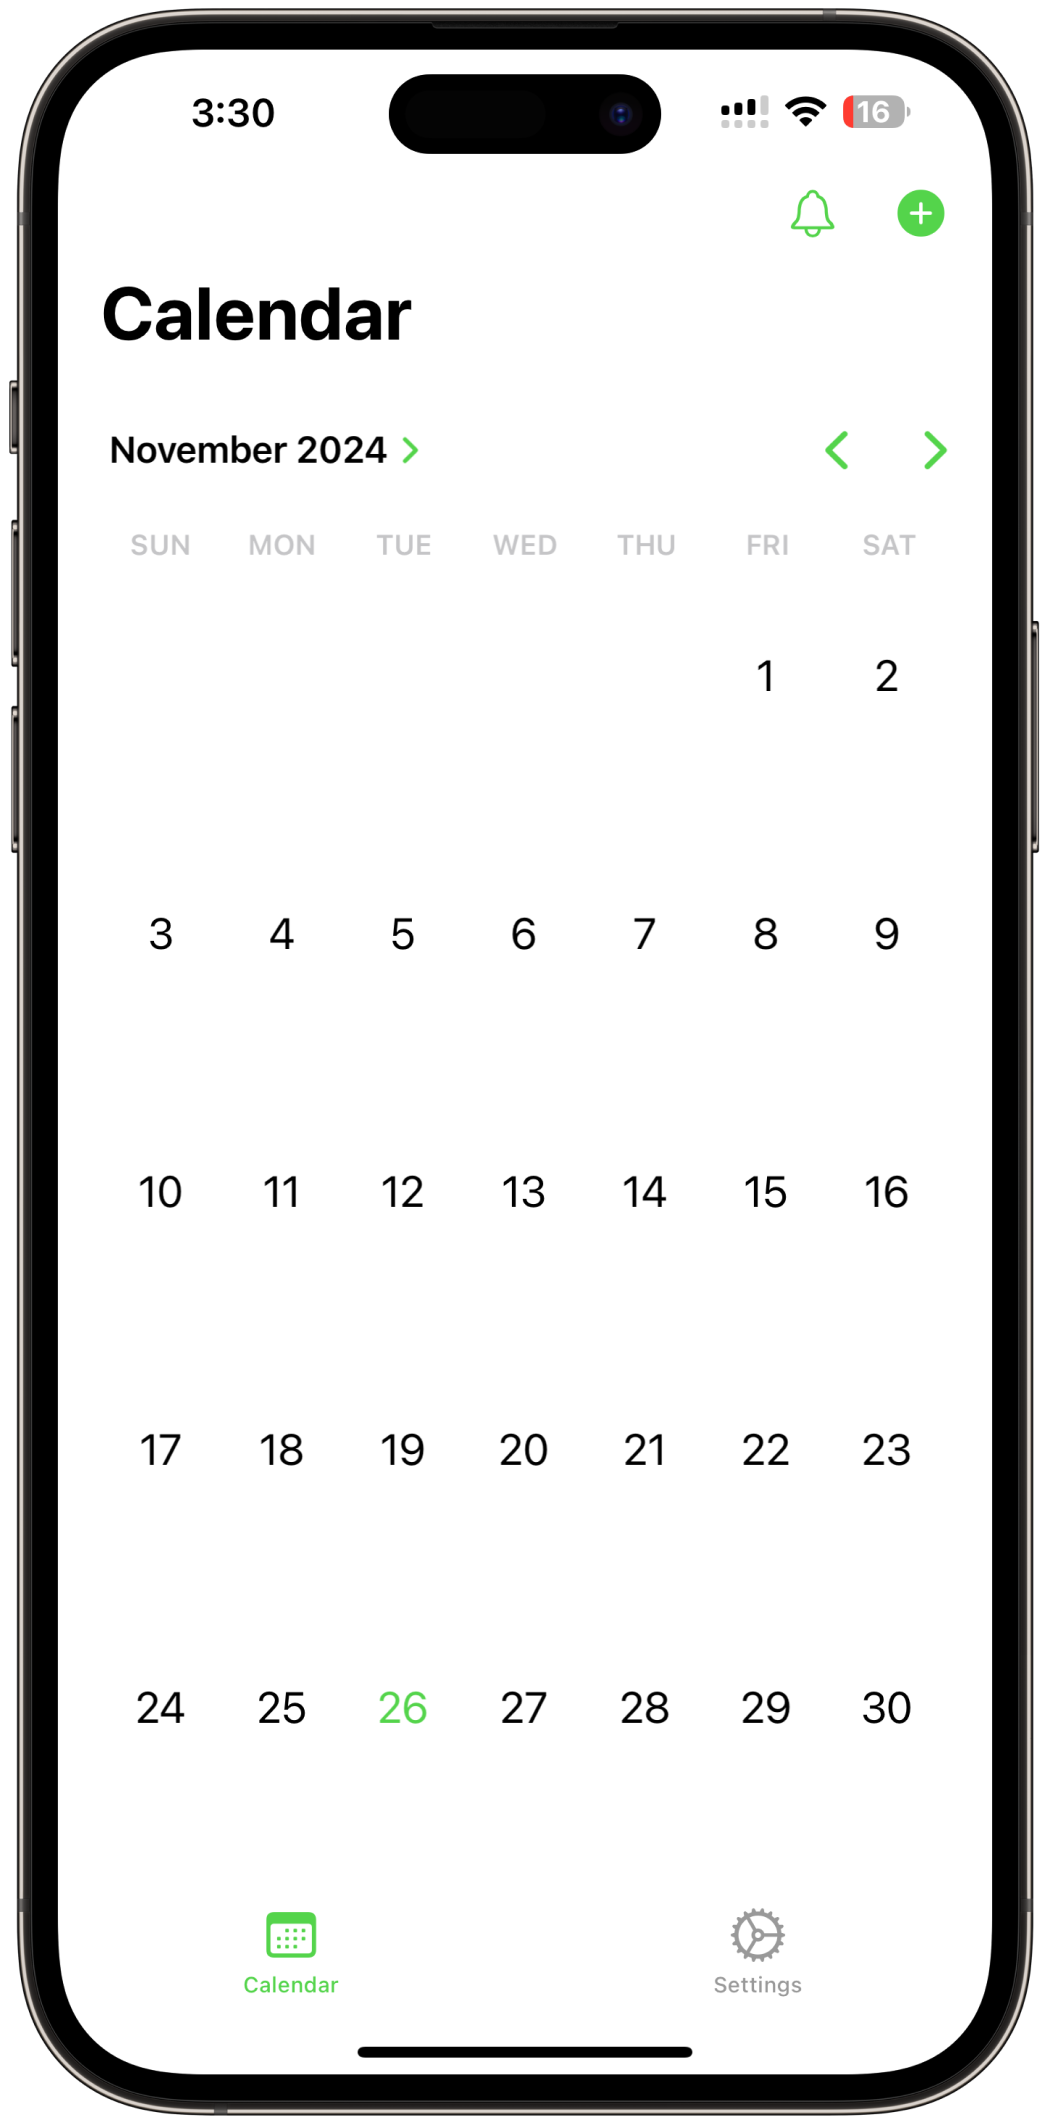
\includegraphics[width=\textwidth]{images/screen1.png}
        \caption{UI Screen 1: Onboarding View}
        \label{fig:ui-screen-1}
    \end{minipage}
    \hfill
    \begin{minipage}{0.65\textwidth}
        In Figure \ref{fig:ui-screen-1}, the screen shows the user the steps he needs to take in the future so he knows what he is going to do. It also has two way of authenticating, Google and Email (Magic Link).
    \end{minipage}
\end{figure}

\begin{figure}[!h]
    \begin{minipage}{0.65\textwidth}
        In Figure \ref{fig:ui-screen-2}, the screen is showing the continue with email screen which allows a user to enter their email, click "Continue", and receive an email if all is good.
    \end{minipage}
    \hfill
    \begin{minipage}{0.3\textwidth}
        \centering
        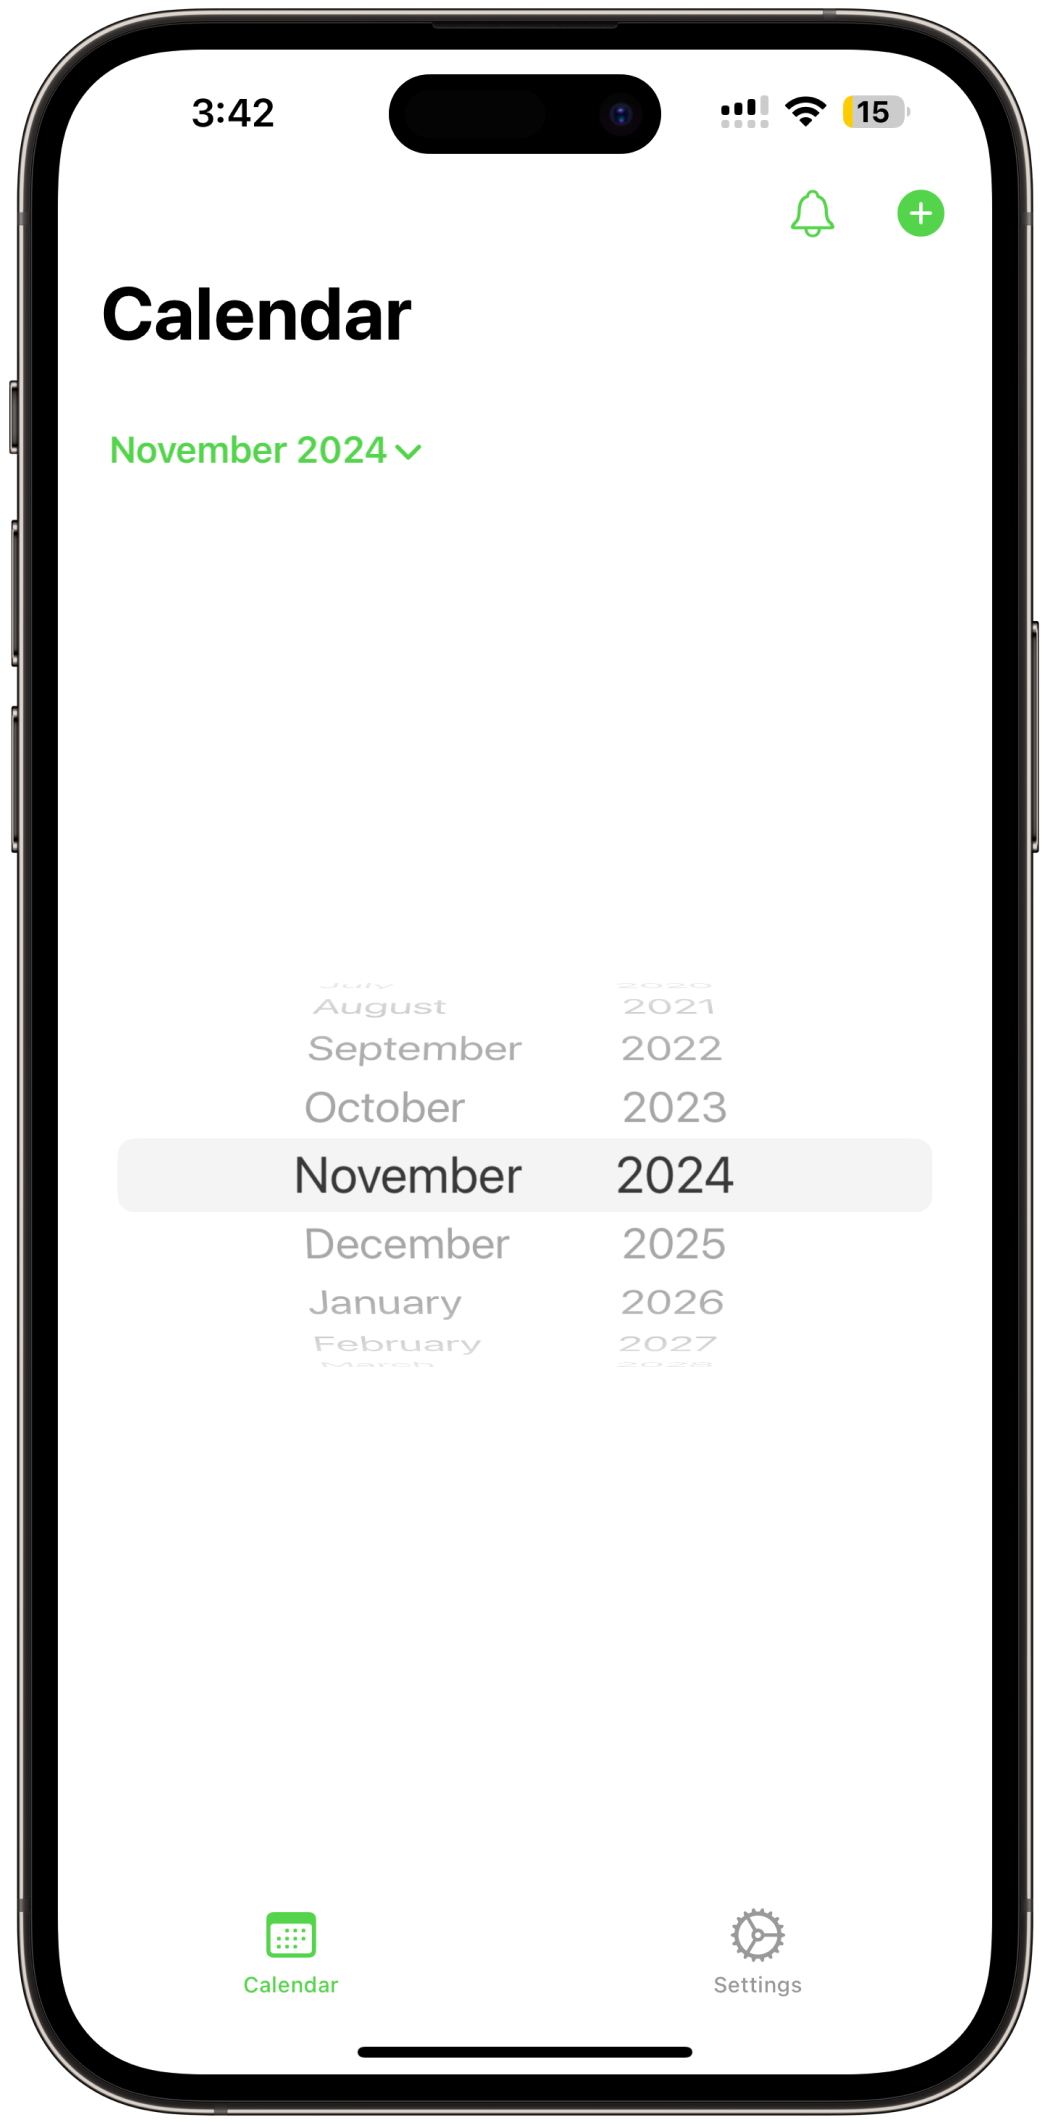
\includegraphics[width=\textwidth]{images/screen2.png}
        \caption{UI Screen 2: Continue with Email View}
        \label{fig:ui-screen-2}
    \end{minipage}
\end{figure}

\begin{figure}[!h]
    \begin{minipage}{0.3\textwidth}
        \centering
        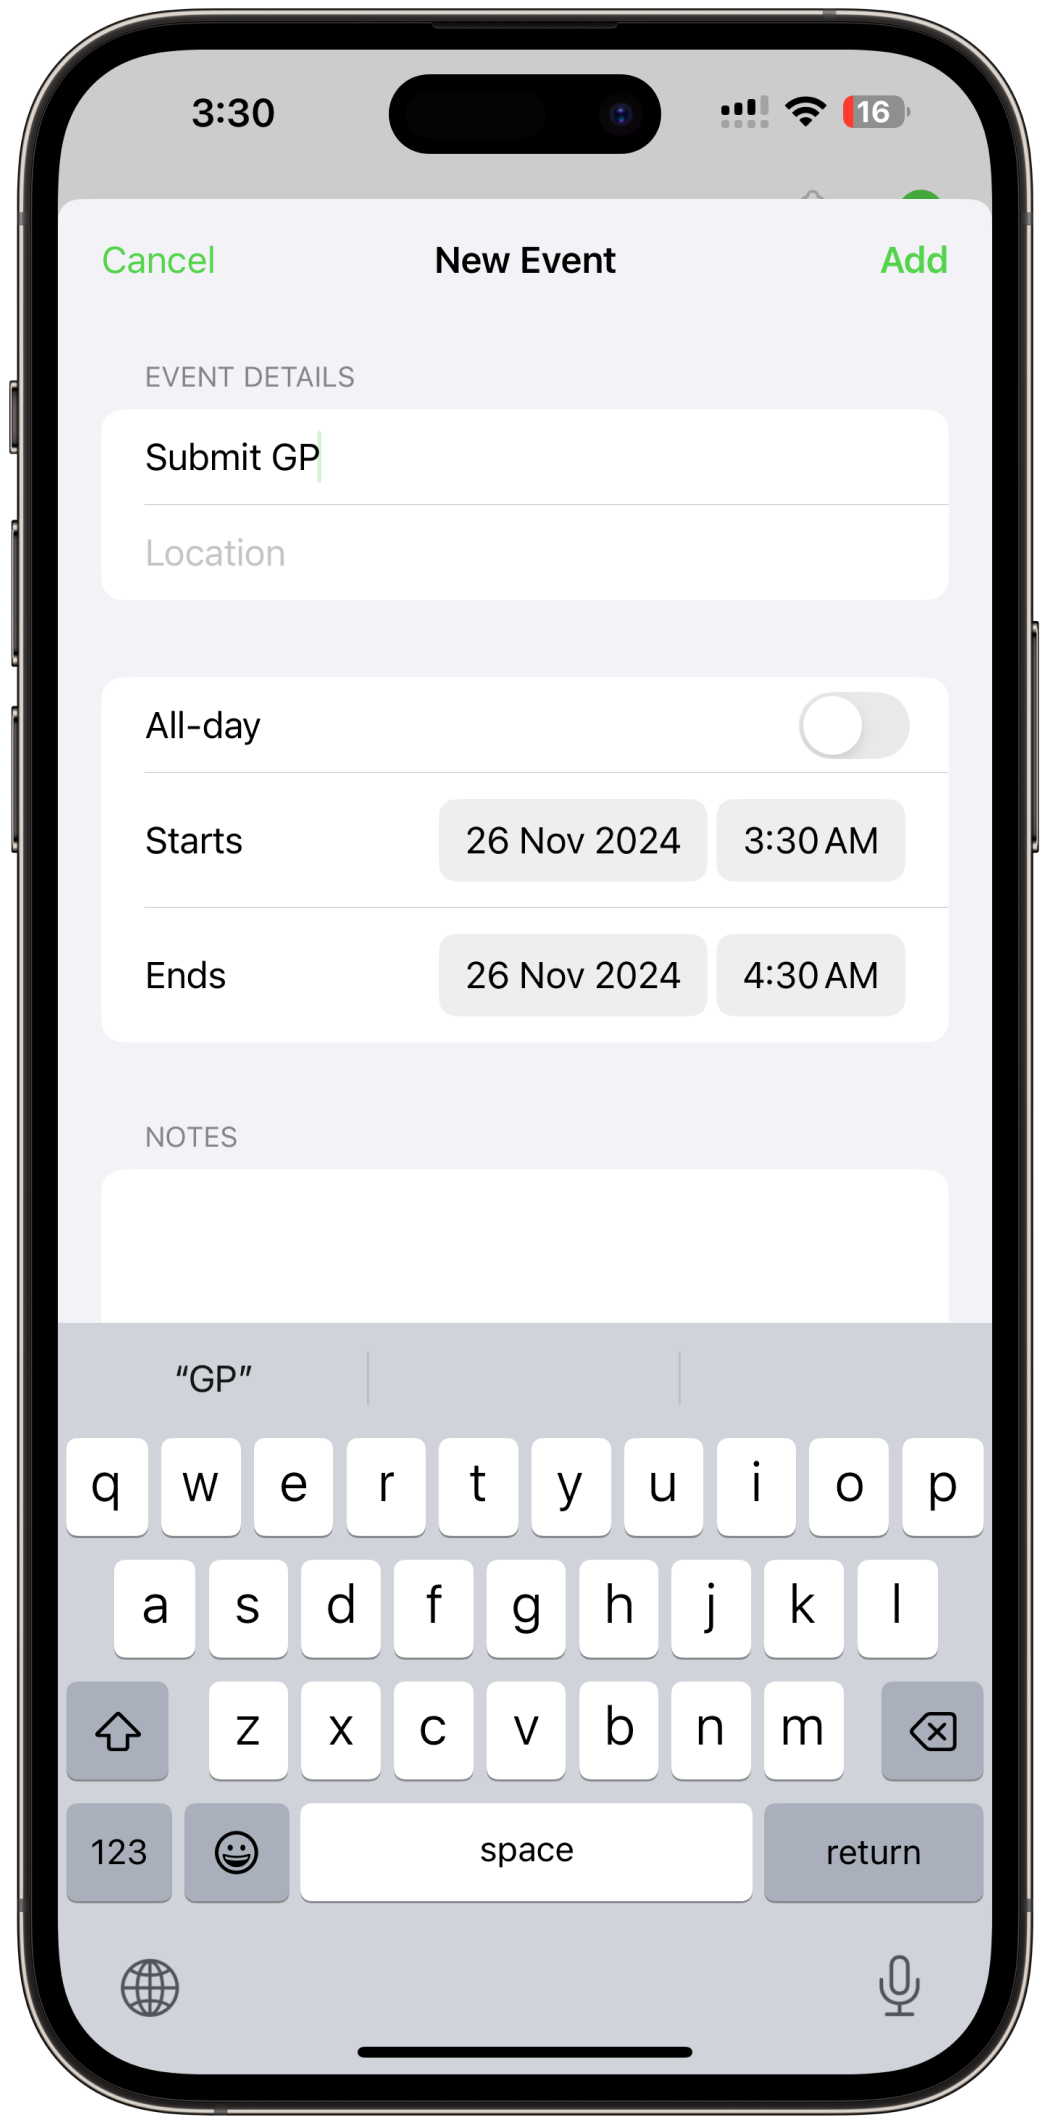
\includegraphics[width=\textwidth]{images/screen3.png}
        \caption{UI Screen 3: Check Your Email View}
        \label{fig:ui-screen-3}
    \end{minipage}
    \hfill
    \begin{minipage}{0.65\textwidth}
        In Figure \ref{fig:ui-screen-3}, the screen that tells the user to check their email for the magic link is shown. They can also click "Resend Email" to get another copy if the first one wasn't received. If they received it, they can click the link inside it and it will redirect back to the app and the app will be able to read the url and its contents which has a token which the app uses to finish the authentication process. Once the authentication process is done, the user is moved to the screen shown in Figure \ref{fig:ui-screen-4}
    \end{minipage}
\end{figure}

\begin{figure}[!h]
    \begin{minipage}{0.65\textwidth}
        In Figure \ref{fig:ui-screen-4}, the calendar view represents the user's schedule. It shows upcoming events, past events, and current events. It also has two buttons at the top, notifications and add event buttons. Users can swipe left and right to navigate months. The current day is colored in green.
    \end{minipage}
    \hfill
    \begin{minipage}{0.3\textwidth}
        \centering
        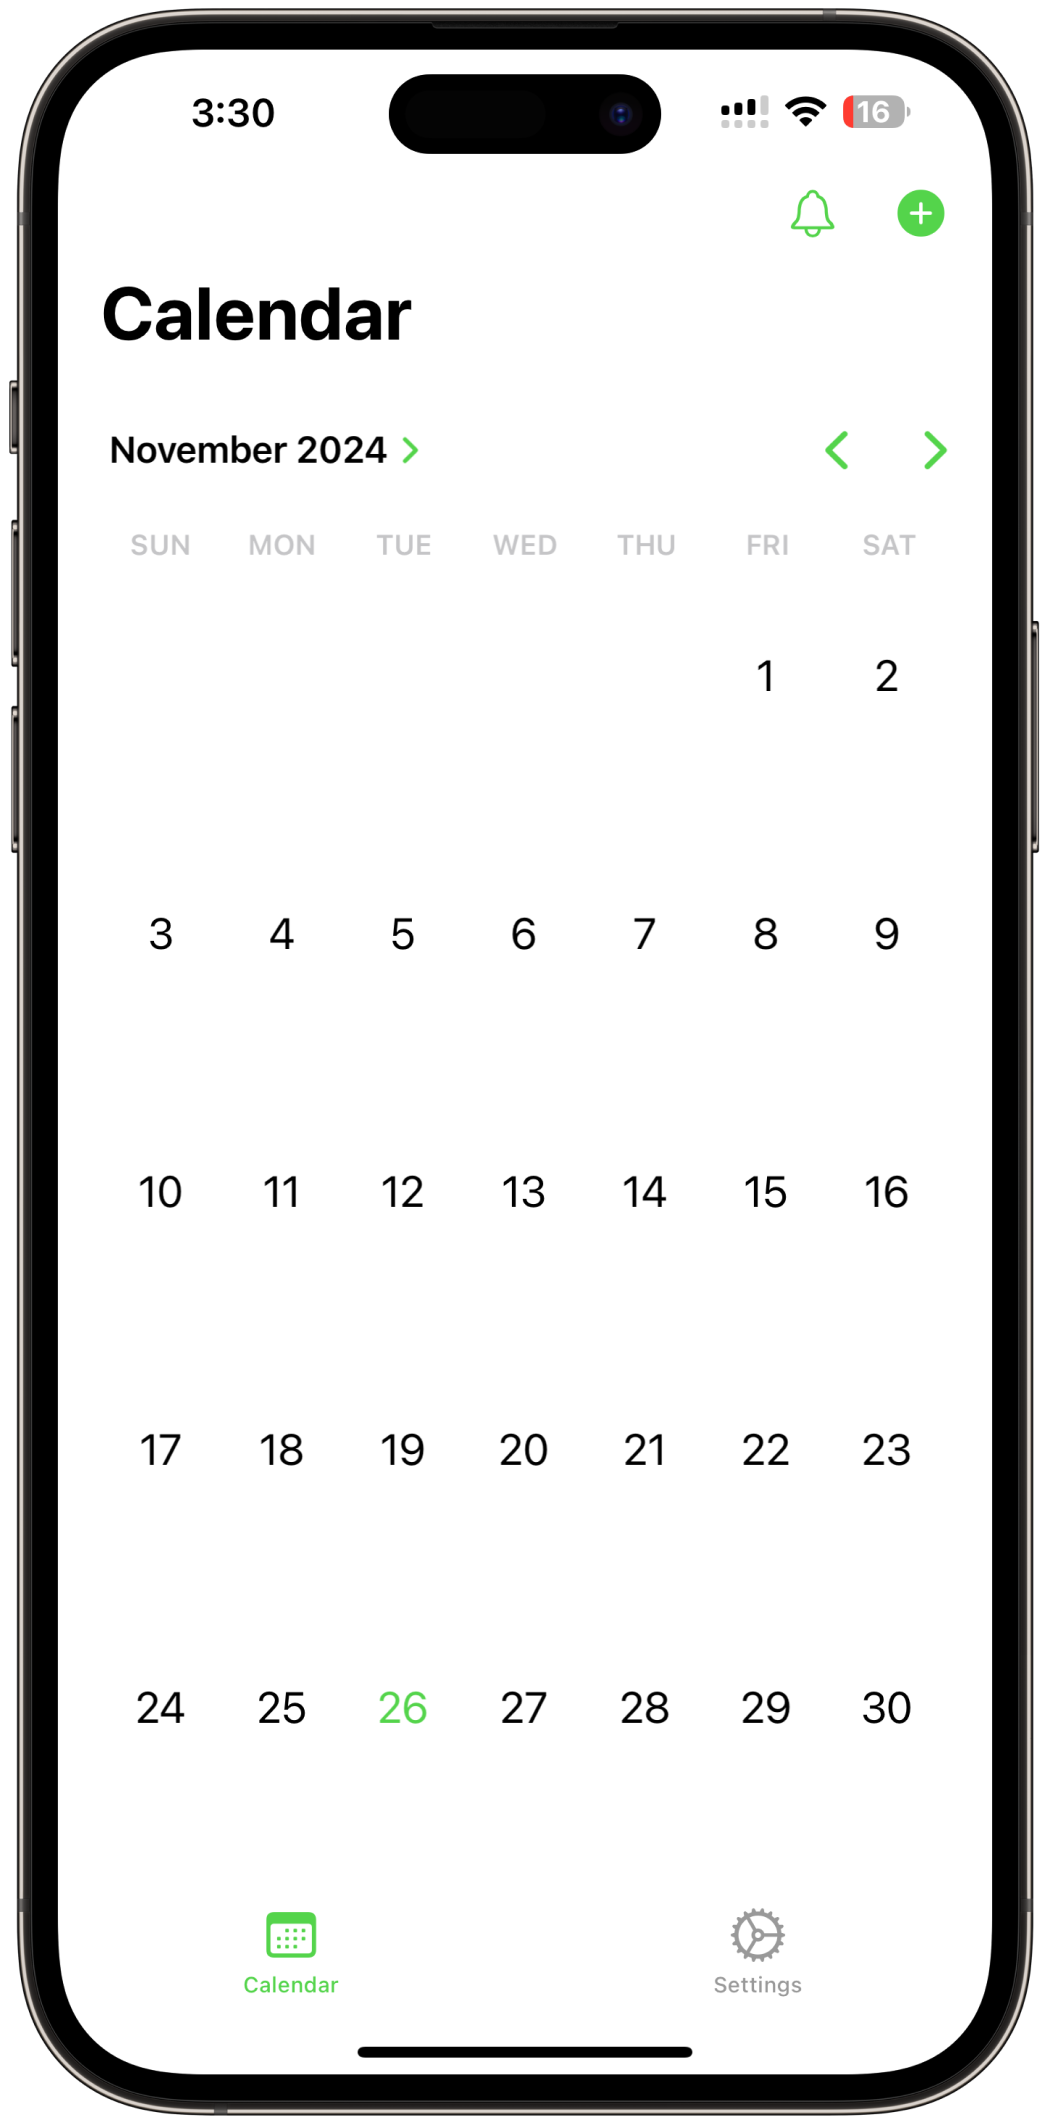
\includegraphics[width=\textwidth]{images/screen4.png}
        \caption{UI Screen 4: Calendar View}
        \label{fig:ui-screen-4}
    \end{minipage}
\end{figure}

\begin{figure}[!h]
    \begin{minipage}{0.3\textwidth}
        \centering
        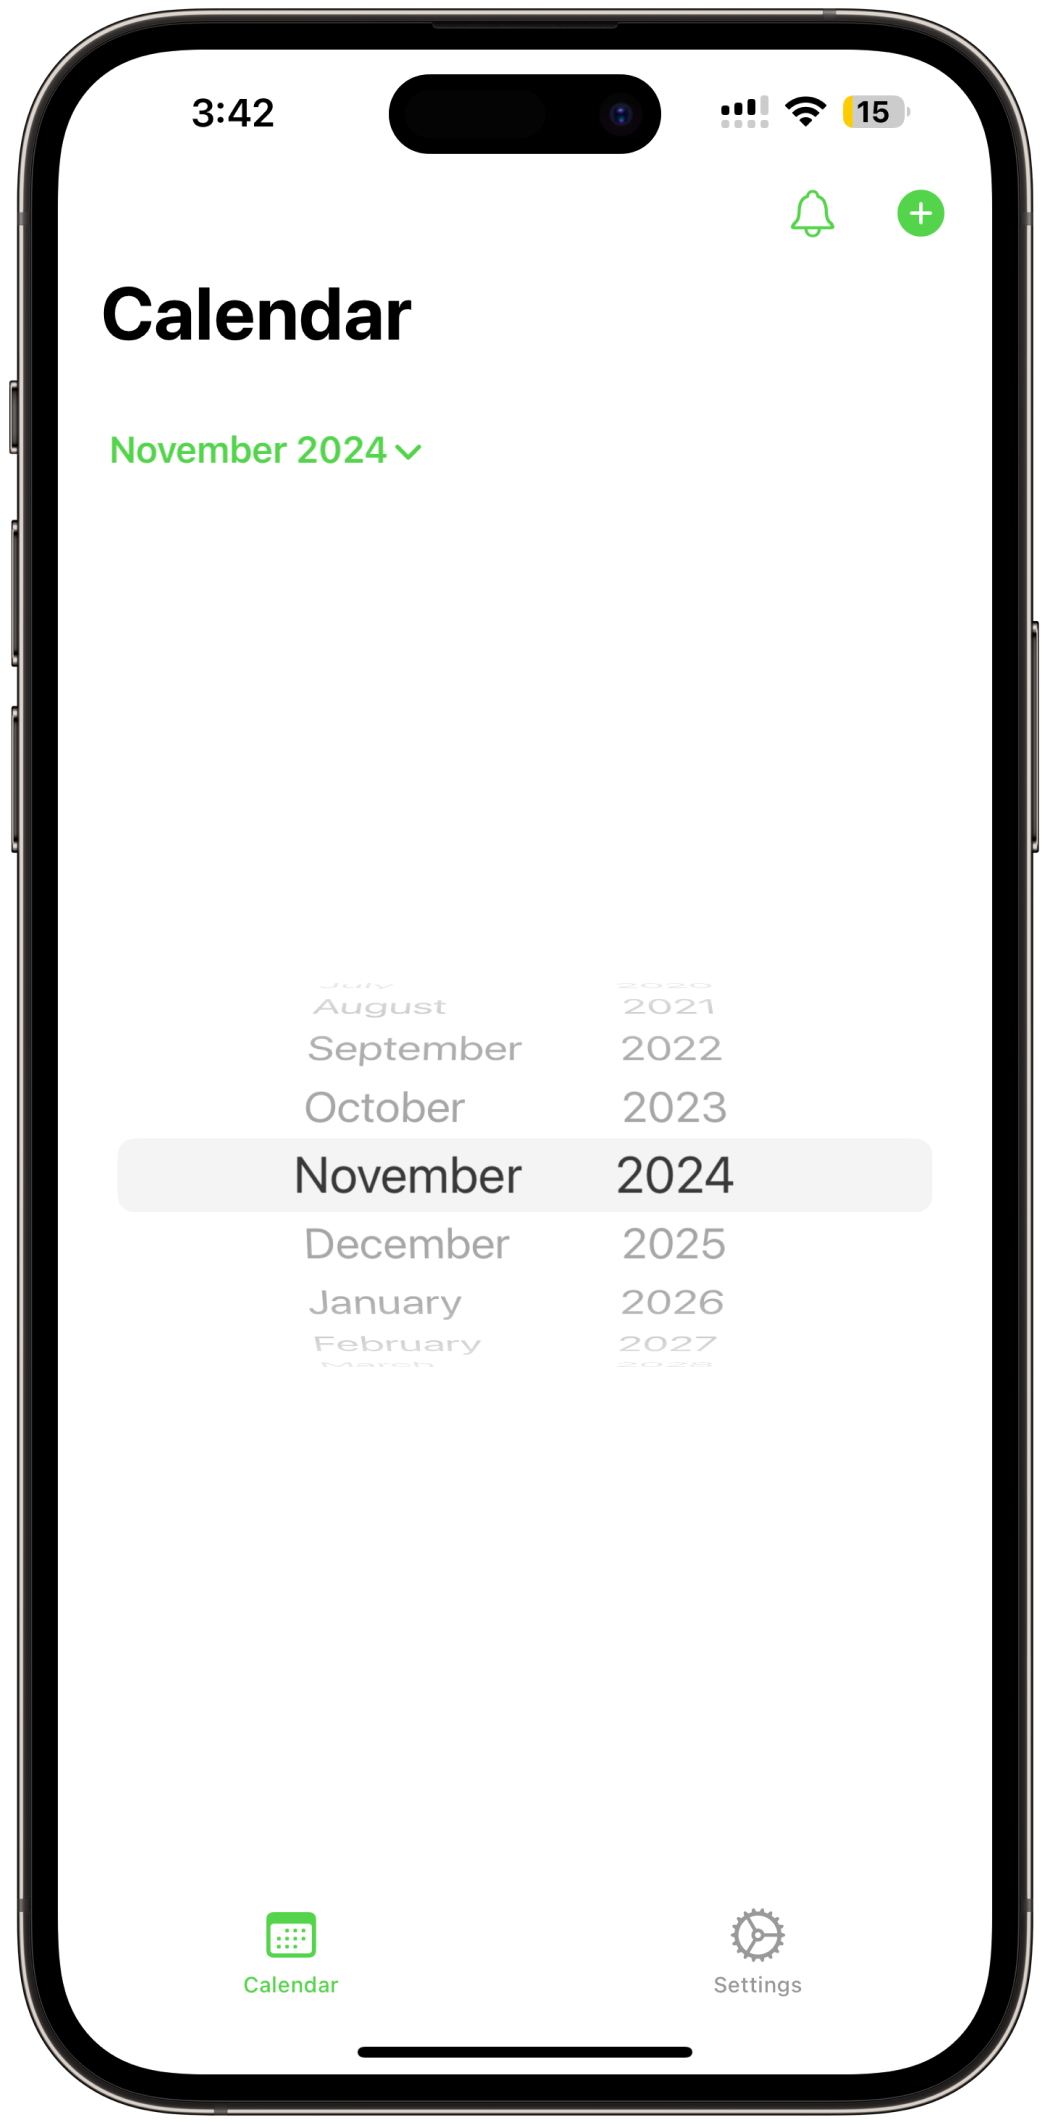
\includegraphics[width=\textwidth]{images/screen5.png}
        \caption{UI Screen 5: Month \& Year Selector}
        \label{fig:ui-screen-5}
    \end{minipage}
    \hfill
    \begin{minipage}{0.65\textwidth}
        In Figure \ref{fig:ui-screen-5}, users can click on the text that shows the currently selected month, in this case ``November 2024'' and get a selector wheel that allows them to choose a month and a year to navigate to.
    \end{minipage}
\end{figure}

\begin{figure}[!h]
    \begin{minipage}{0.65\textwidth}
        In Figure \ref{fig:ui-screen-6}, the screen is showing the add event sheet in its default state. It is shown when you click the "add event" button in Figure \ref{fig:ui-screen-4}.
    \end{minipage}
    \hfill
    \begin{minipage}{0.3\textwidth}
        \centering
        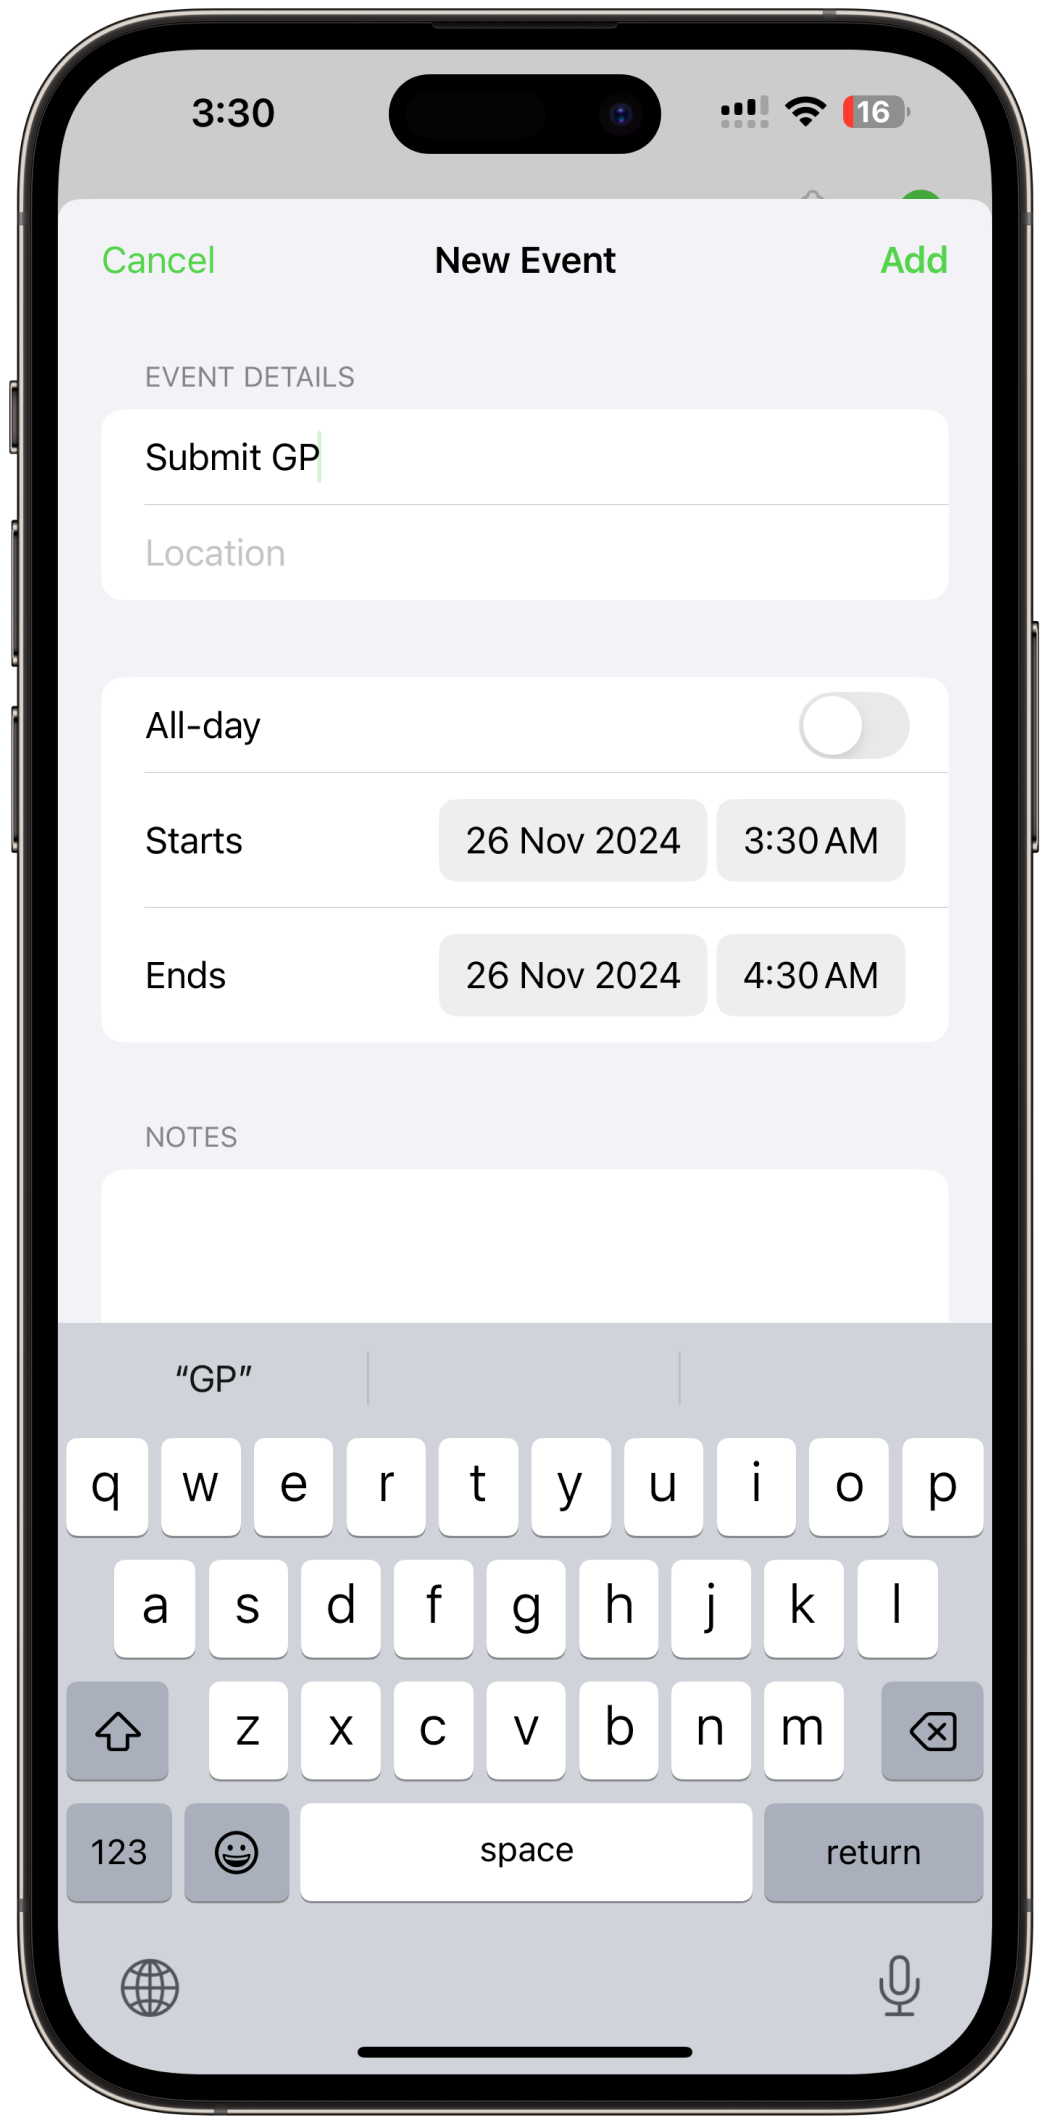
\includegraphics[width=\textwidth]{images/screen6.png}
        \caption{UI Screen 6: Add Event View - Default}
        \label{fig:ui-screen-6}
    \end{minipage}
\end{figure}

\begin{figure}[!h]
    \begin{minipage}{0.3\textwidth}
        \centering
        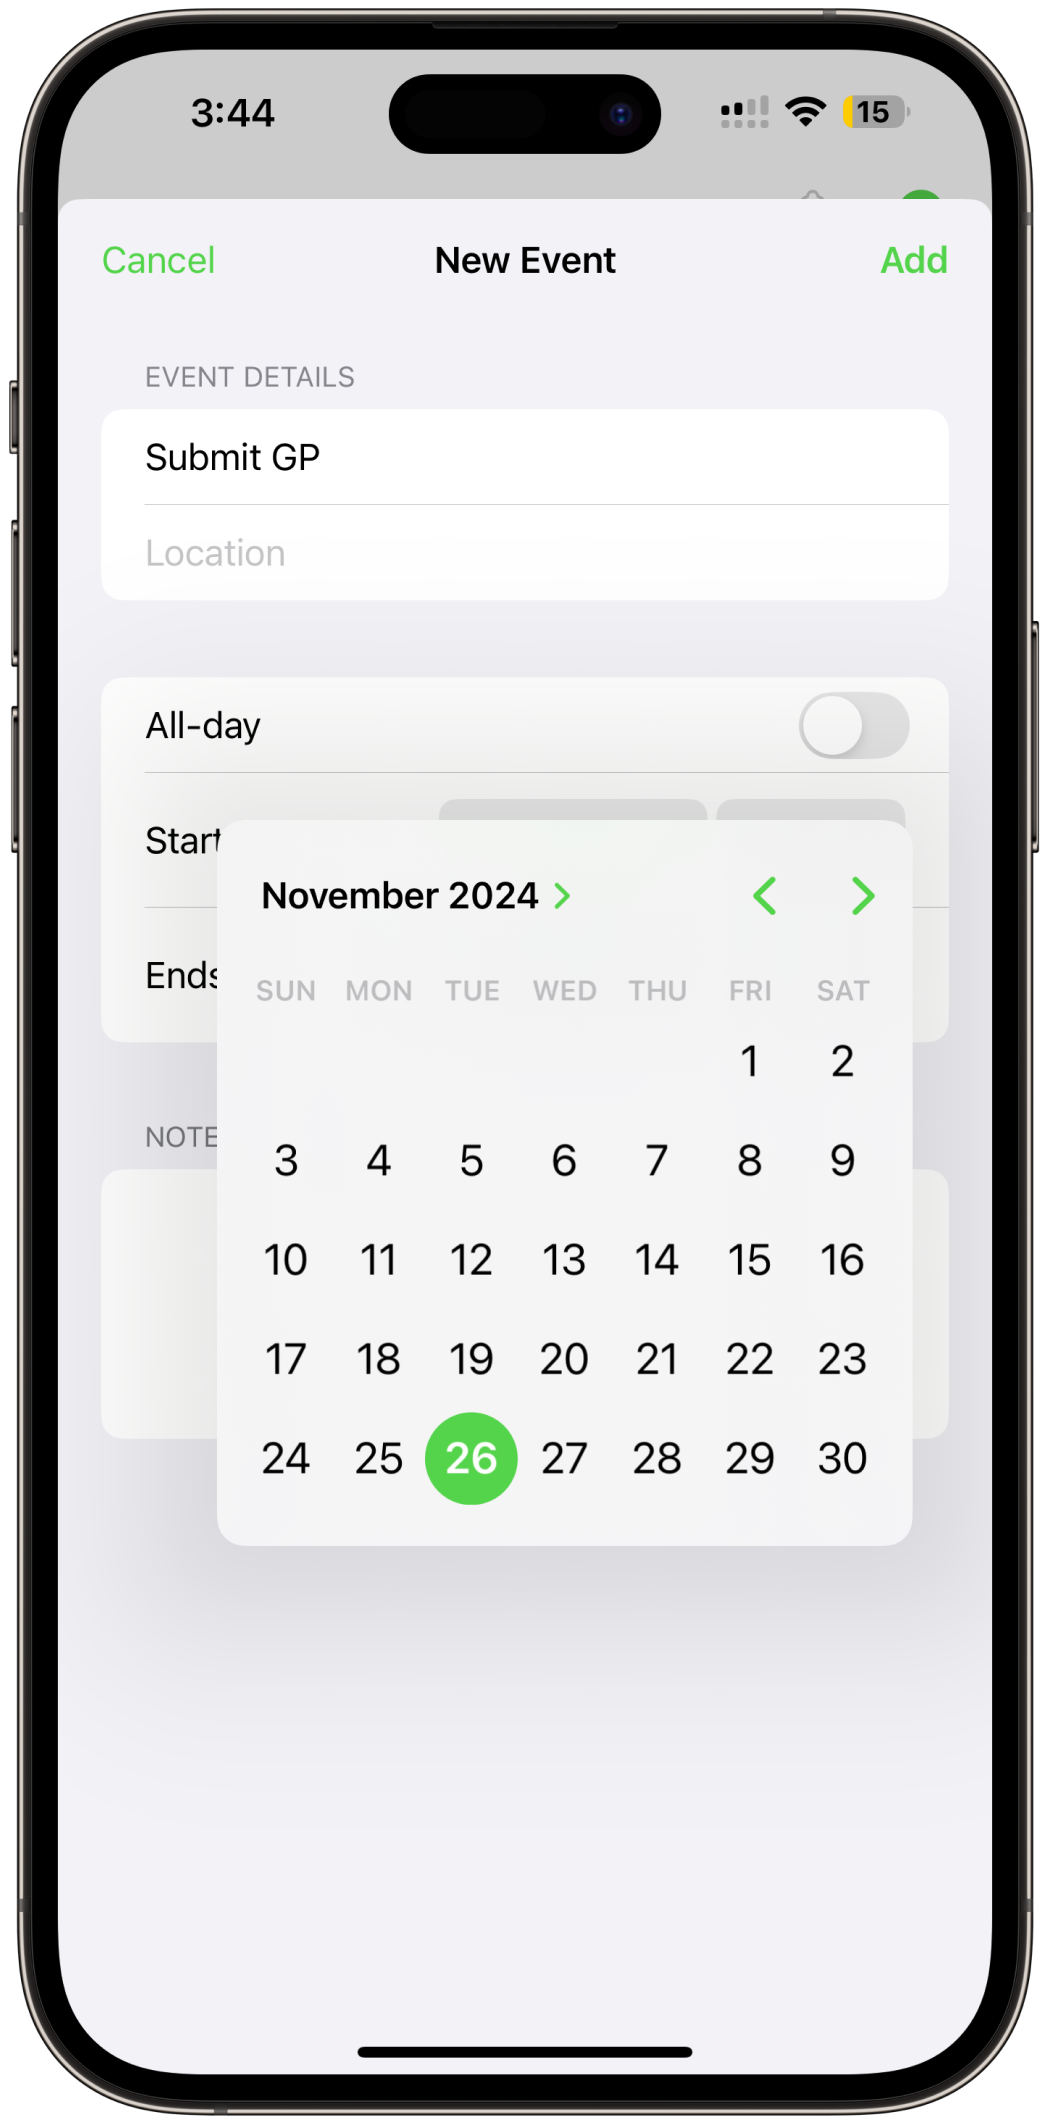
\includegraphics[width=\textwidth]{images/screen7.png}
        \caption{UI Screen 7: Add Event View - Date Picker}
        \label{fig:ui-screen-7}
    \end{minipage}
    \hfill
    \begin{minipage}{0.65\textwidth}
        In Figure \ref{fig:ui-screen-7}, the screen is showing the add event sheet in its date picker chosen state. You can choose a date and scroll between months and years if you want.
    \end{minipage}
\end{figure}

\begin{figure}[!h]
    \begin{minipage}{0.65\textwidth}
        In Figure \ref{fig:ui-screen-8}, the screen is showing the add event sheet in its time picker chosen state. You can choose a time and scroll between hours and minutes if you want.
    \end{minipage}
    \hfill
    \begin{minipage}{0.3\textwidth}
        \centering
        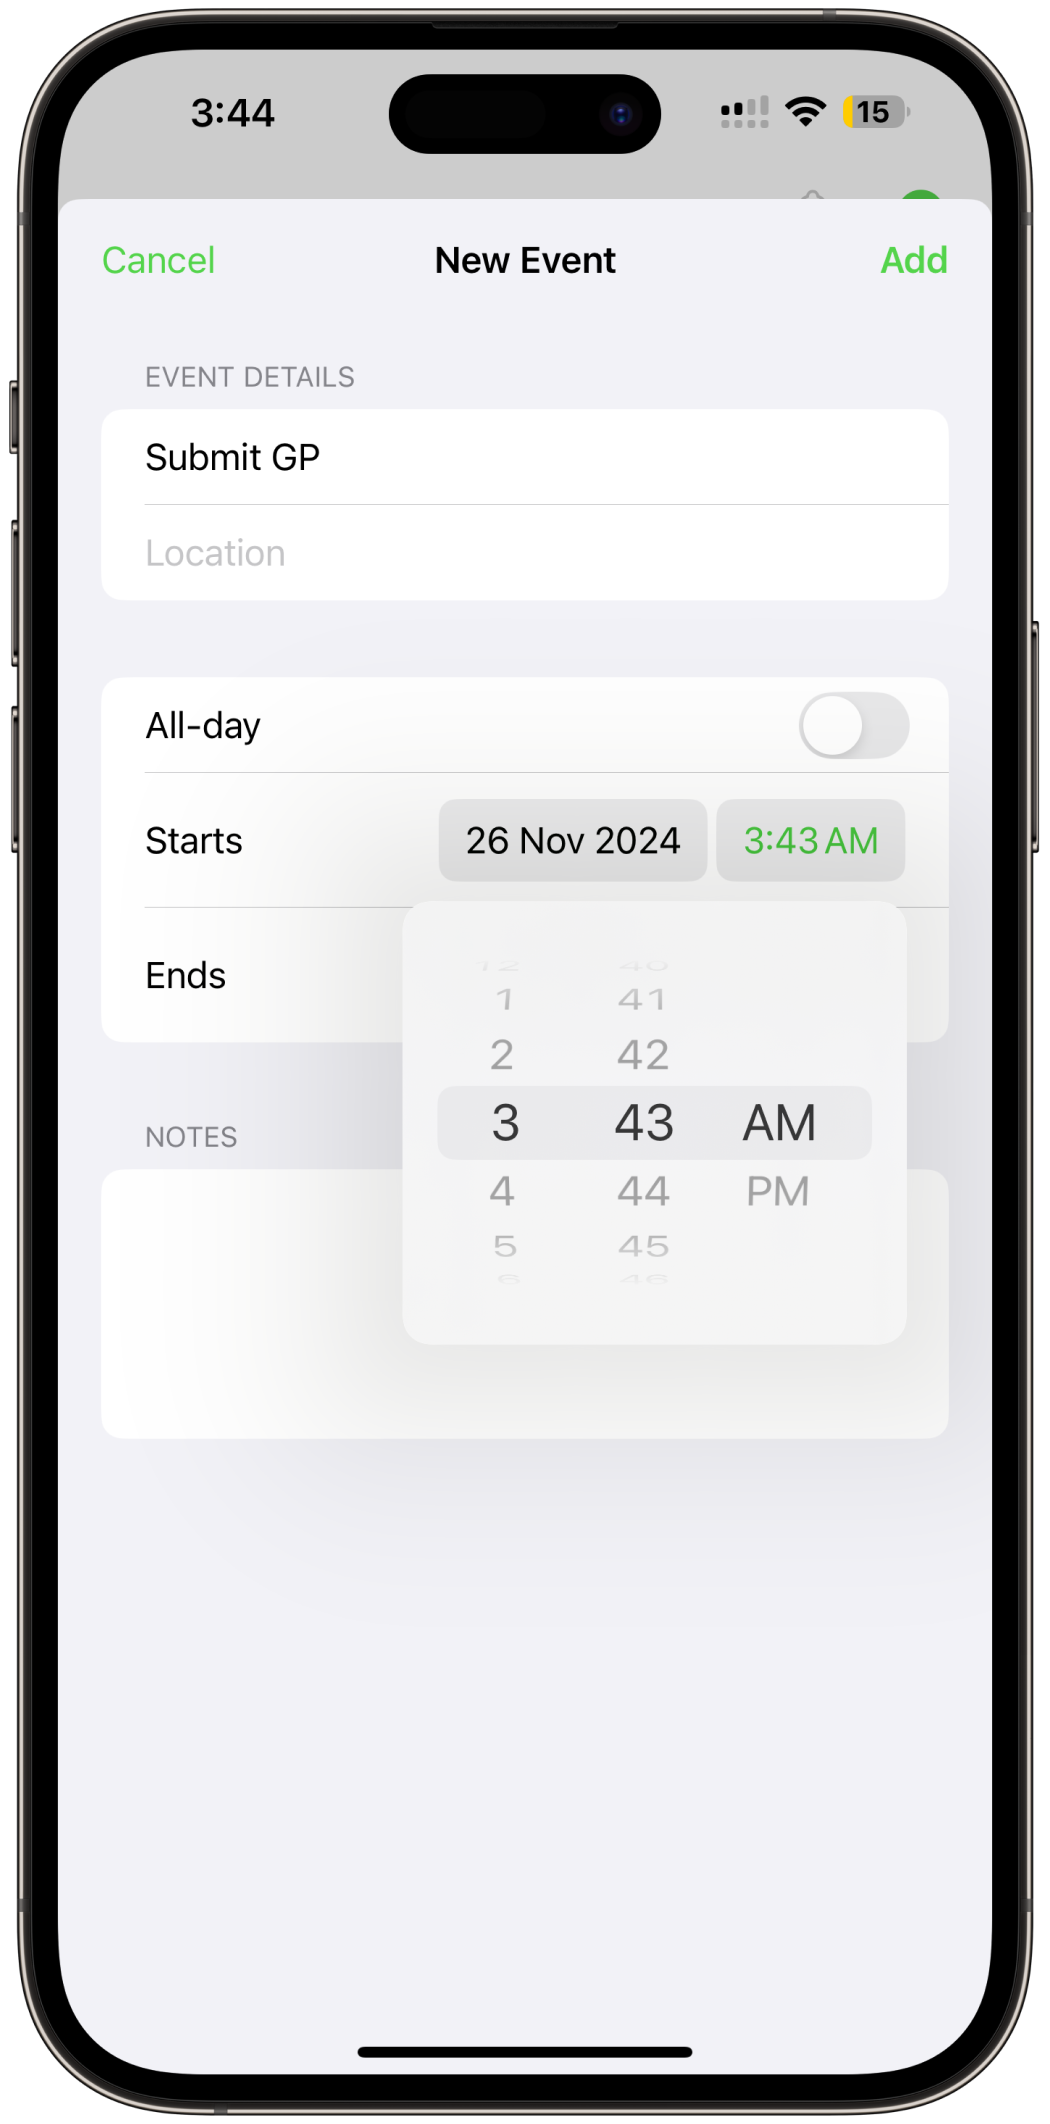
\includegraphics[width=\textwidth]{images/screen8.png}
        \caption{UI Screen 8: Add Event View - Time Picker}
        \label{fig:ui-screen-8}
    \end{minipage}
\end{figure}

\begin{figure}[!h]
    \begin{minipage}{0.3\textwidth}
        \centering
        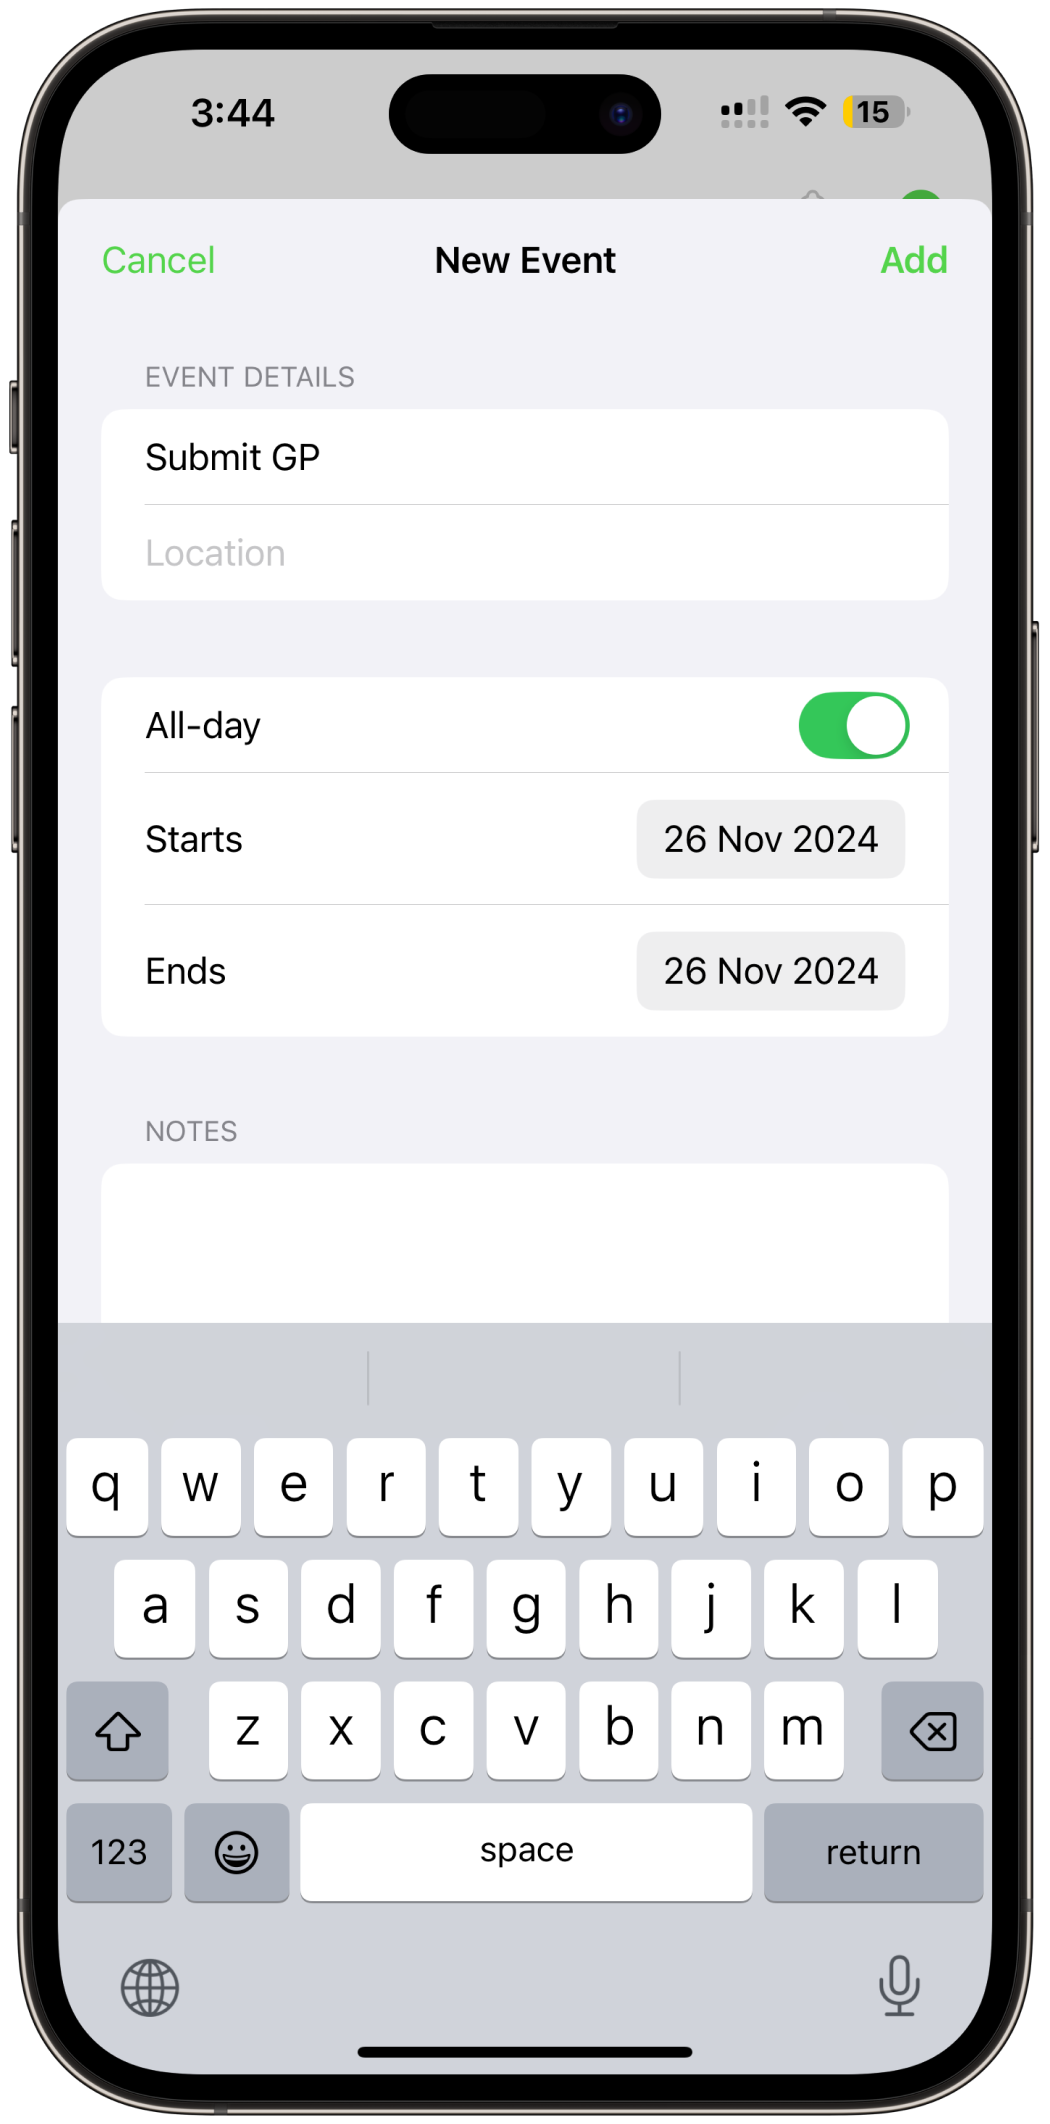
\includegraphics[width=\textwidth]{images/screen9.png}
        \caption{UI Screen 9: Add Event View - All Day}
        \label{fig:ui-screen-9}
    \end{minipage}
    \hfill
    \begin{minipage}{0.65\textwidth}
        In Figure \ref{fig:ui-screen-9}, the settings page is shown. This pae has the user details, specifcally email, and name. Also the "Connect WhatsApp" button is shown along with the "Connect CalDAV" button. Those two buttons do as they say and allow users to have data sources for the calendar connected. The last button shown is the logout button, and this button is in red to make the user alerted and not click it by mistake. Clicking it will log the user out and take them to the home screen.
    \end{minipage}
\end{figure}

\begin{figure}[!h]
    \begin{minipage}{0.65\textwidth}
        In Figure \ref{fig:ui-screen-10}, the settings page is shown. This pae has the user details, specifcally email, and name. Also the "Connect WhatsApp" button is shown along with the "Connect CalDAV" button. Those two buttons do as they say and allow users to have data sources for the calendar connected. The last button shown is the logout button, and this button is in red to make the user alerted and not click it by mistake. Clicking it will log the user out and take them to the home screen.
    \end{minipage}
    \hfill
    \begin{minipage}{0.3\textwidth}
        \centering
        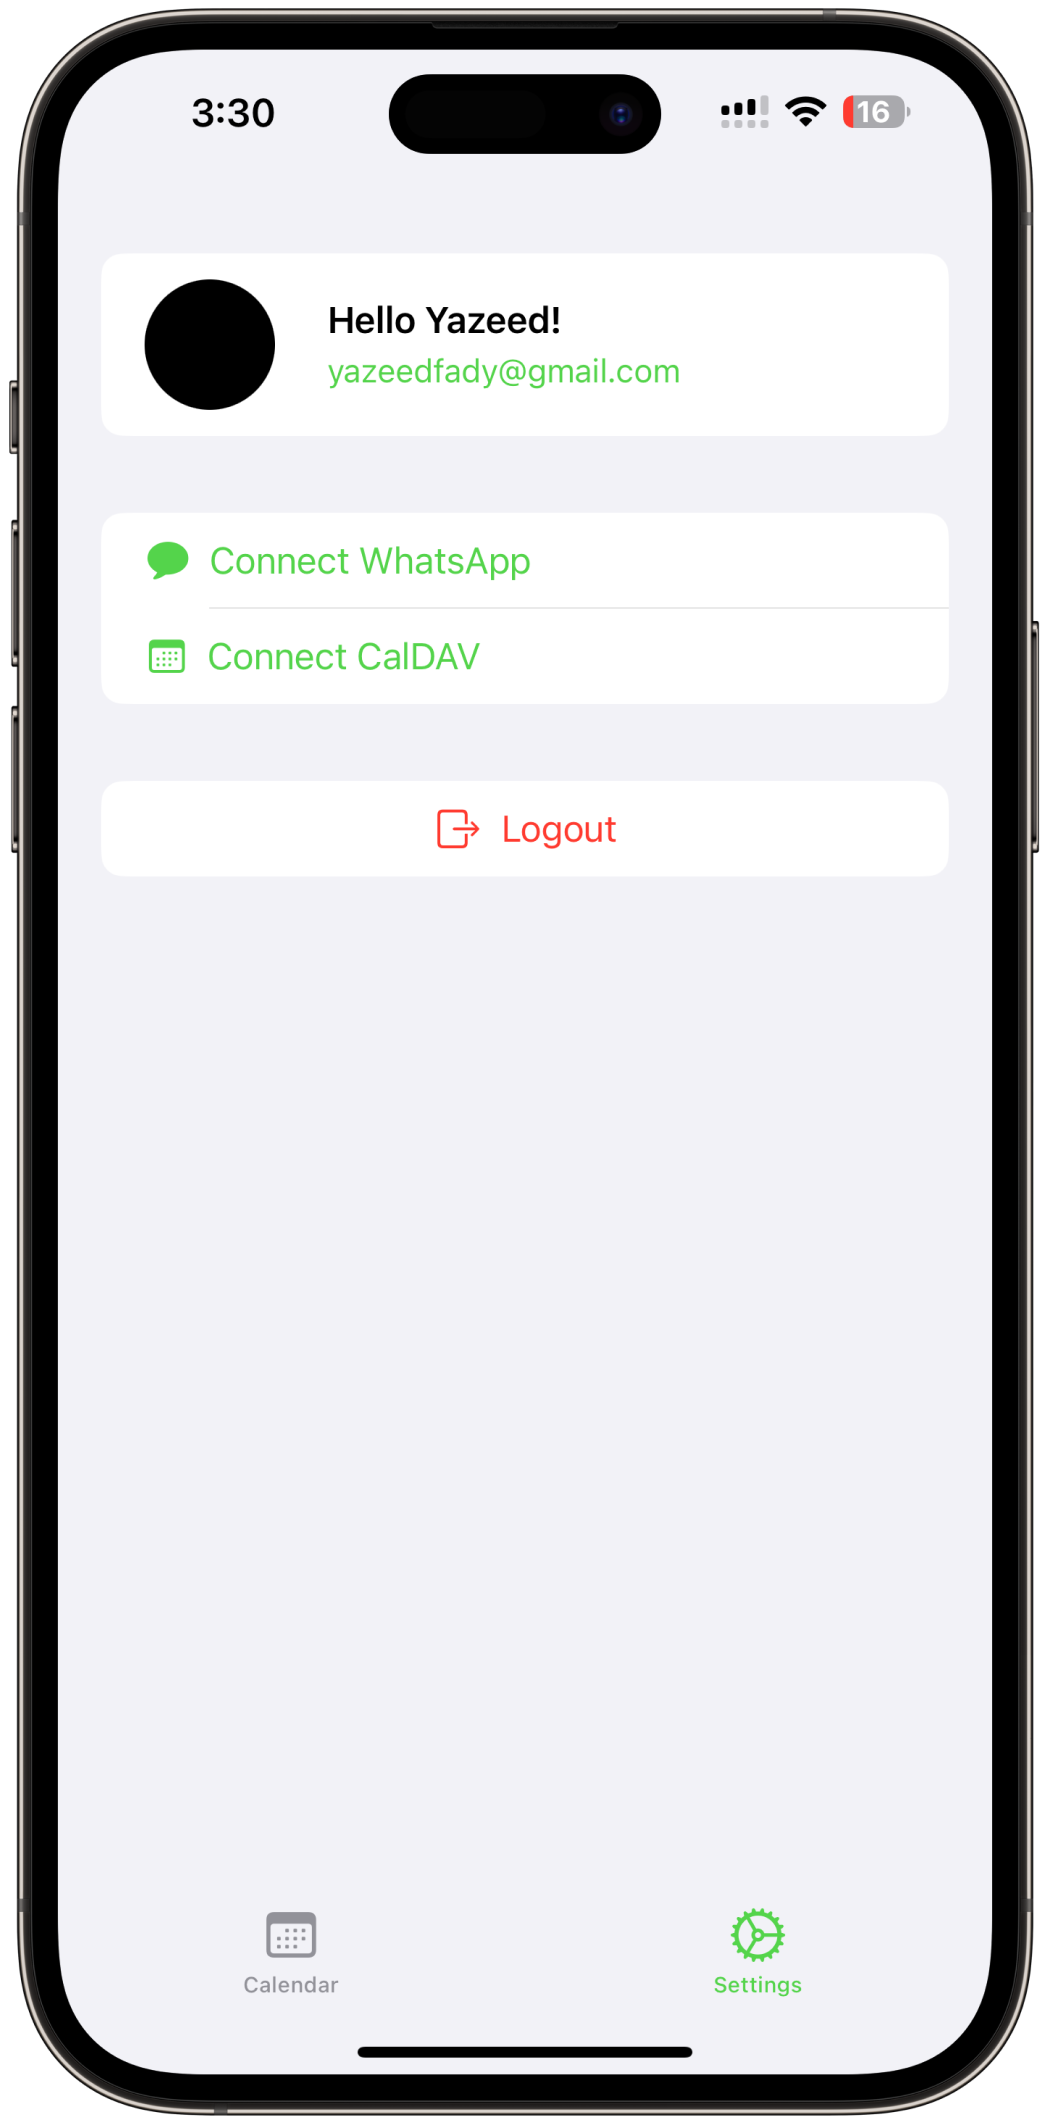
\includegraphics[width=\textwidth]{images/screen10.png}
        \caption{UI Screen 10: Settings View}
        \label{fig:ui-screen-10}
    \end{minipage}
\end{figure}